\documentclass[a4paper]{article}\usepackage[]{graphicx}\usepackage[]{color}
%% maxwidth is the original width if it is less than linewidth
%% otherwise use linewidth (to make sure the graphics do not exceed the margin)
\makeatletter
\def\maxwidth{ %
  \ifdim\Gin@nat@width>\linewidth
    \linewidth
  \else
    \Gin@nat@width
  \fi
}
\makeatother

\definecolor{fgcolor}{rgb}{0.345, 0.345, 0.345}
\newcommand{\hlnum}[1]{\textcolor[rgb]{0.686,0.059,0.569}{#1}}%
\newcommand{\hlstr}[1]{\textcolor[rgb]{0.192,0.494,0.8}{#1}}%
\newcommand{\hlcom}[1]{\textcolor[rgb]{0.678,0.584,0.686}{\textit{#1}}}%
\newcommand{\hlopt}[1]{\textcolor[rgb]{0,0,0}{#1}}%
\newcommand{\hlstd}[1]{\textcolor[rgb]{0.345,0.345,0.345}{#1}}%
\newcommand{\hlkwa}[1]{\textcolor[rgb]{0.161,0.373,0.58}{\textbf{#1}}}%
\newcommand{\hlkwb}[1]{\textcolor[rgb]{0.69,0.353,0.396}{#1}}%
\newcommand{\hlkwc}[1]{\textcolor[rgb]{0.333,0.667,0.333}{#1}}%
\newcommand{\hlkwd}[1]{\textcolor[rgb]{0.737,0.353,0.396}{\textbf{#1}}}%

\usepackage{framed}
\makeatletter
\newenvironment{kframe}{%
 \def\at@end@of@kframe{}%
 \ifinner\ifhmode%
  \def\at@end@of@kframe{\end{minipage}}%
  \begin{minipage}{\columnwidth}%
 \fi\fi%
 \def\FrameCommand##1{\hskip\@totalleftmargin \hskip-\fboxsep
 \colorbox{shadecolor}{##1}\hskip-\fboxsep
     % There is no \\@totalrightmargin, so:
     \hskip-\linewidth \hskip-\@totalleftmargin \hskip\columnwidth}%
 \MakeFramed {\advance\hsize-\width
   \@totalleftmargin\z@ \linewidth\hsize
   \@setminipage}}%
 {\par\unskip\endMakeFramed%
 \at@end@of@kframe}
\makeatother

\definecolor{shadecolor}{rgb}{.97, .97, .97}
\definecolor{messagecolor}{rgb}{0, 0, 0}
\definecolor{warningcolor}{rgb}{1, 0, 1}
\definecolor{errorcolor}{rgb}{1, 0, 0}
\newenvironment{knitrout}{}{} % an empty environment to be redefined in TeX

\usepackage{alltt}
\usepackage[margin=2cm]{geometry}
\usepackage{graphicx, subfig}


\usepackage[british]{babel}
\usepackage{enumerate}
\IfFileExists{upquote.sty}{\usepackage{upquote}}{}
\begin{document}
\title{STAT 640 || Assignment 2}
%\subtitle{Homework 2}
\author{SD }
\maketitle

\section{ Exercise 9.1(1)}

Johnson et al. (1970) considered the behavior of a cenosphere-resin composite under
hydrostatic pressure. The authors pointed out that most deep submersible vehicles utilize a
buoyancy material, known as syntactic foam, that is a composite of closely packed hollow
glass microspheres embedded in a resin matrix. These microspheres are relatively expensive
to manufacture, and the cost of the syntactic foam is principally determined by the cost of the microspheres. The authors also noted that the ash from generating stations burning pulverized coal contains a small proportion of hollow glassy microspheres, known as cenospheres, and these have about the right size distribution for use in syntactic foam. The cenospheres can be readily collected from the ash-disposal method used in certain British generating stations. The authors were thus interested in whether the cenospheres would, in some applications, perform as well as the manufactured microspheres.\\
In attempting to assess the usefulness of cenospheres as a component of syntactic foam,
Johnson et al. investigated the effects of hydrostatic pressure (such as exists in the ocean
depths) on the density of a cenosphere-resin composite. The results are given in Table 9.2.
What is the P-value for a test of $H_0: \beta= 0$ against the alternative $H_1: \beta > 0$ for these data?\\

\vspace{2 mm}

\raggedright{\textbf{Solution:}}\\

\begin{knitrout}
\definecolor{shadecolor}{rgb}{0.969, 0.969, 0.969}\color{fgcolor}\begin{kframe}
\begin{alltt}
\hlstd{X} \hlkwb{<-} \hlkwd{c}\hlstd{(}\hlnum{0}\hlstd{,} \hlnum{5000}\hlstd{,} \hlnum{10000}\hlstd{,} \hlnum{15000}\hlstd{,} \hlnum{20000}\hlstd{,} \hlnum{25000}\hlstd{,} \hlnum{30000}\hlstd{,} \hlnum{100000} \hlstd{)}
\hlstd{Y} \hlkwb{<-} \hlkwd{c}\hlstd{(}\hlnum{0.924}\hlstd{,} \hlnum{0.988}\hlstd{,} \hlnum{0.992}\hlstd{,} \hlnum{1.118}\hlstd{,} \hlnum{1.133}\hlstd{,} \hlnum{1.145}\hlstd{,} \hlnum{1.157}\hlstd{,} \hlnum{1.357}\hlstd{)}
\hlstd{dat} \hlkwb{<-} \hlkwd{data.frame}\hlstd{(X, Y)}
\hlstd{dat}
\end{alltt}
\begin{verbatim}
##        X     Y
## 1      0 0.924
## 2   5000 0.988
## 3  10000 0.992
## 4  15000 1.118
## 5  20000 1.133
## 6  25000 1.145
## 7  30000 1.157
## 8 100000 1.357
\end{verbatim}
\begin{alltt}
\hlkwd{library}\hlstd{(NSM3)}
\end{alltt}


{\ttfamily\noindent\itshape\color{messagecolor}{\#\# Loading required package: combinat\\\#\# \\\#\# Attaching package: 'combinat'\\\#\# \\\#\# The following object is masked from 'package:utils':\\\#\# \\\#\#\ \ \ \  combn\\\#\# \\\#\# Loading required package: MASS\\\#\# Loading required package: partitions\\\#\# Loading required package: survival\\\#\# Loading required package: splines\\\#\# fANCOVA 0.5-1 loaded}}\begin{alltt}
\hlkwd{theil}\hlstd{(X, Y,} \hlkwc{beta.0}\hlstd{=}\hlnum{0}\hlstd{,} \hlkwc{type}\hlstd{=}\hlstr{"u"}\hlstd{)}
\end{alltt}
\begin{verbatim}
## 
## Null: beta greater than 0
## C = 28, C.bar = 1, P = 0
## beta.hat = 0
## alpha.hat = 0.975
## 
## 1 - alpha = 0.95 upper bound for beta:
## -Inf, 0
\end{verbatim}
\end{kframe}
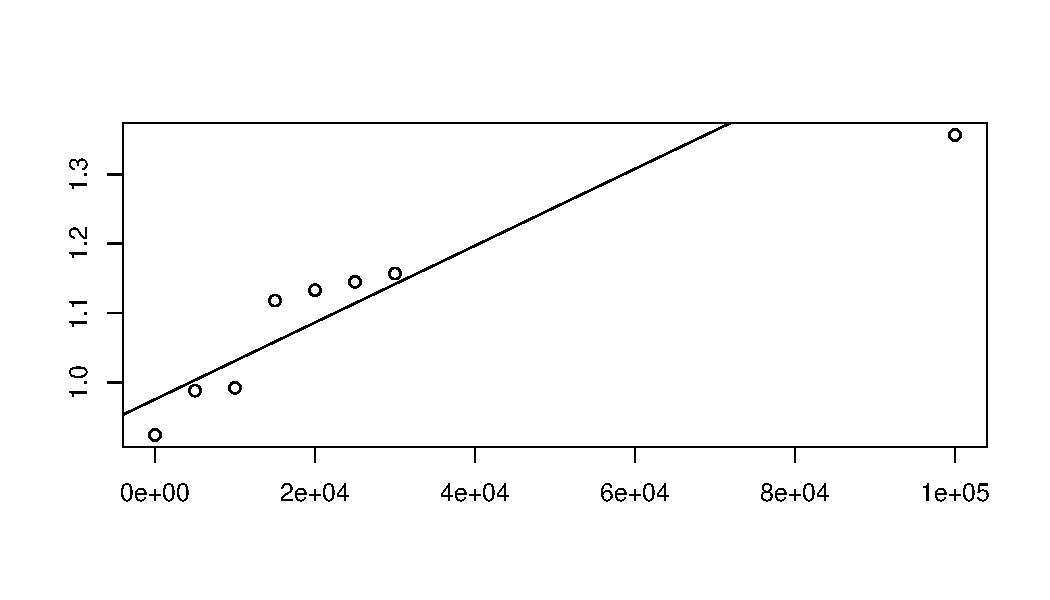
\includegraphics[width=\maxwidth]{figure/unnamed-chunk-1-1} 

\end{knitrout}
\raggedright{From the Theil function we find that p=0 (which is less than 0.05). We fail to reject the null hupothesis.}\\


\vspace{2 mm}

\section{ Exercise 9.2(7)}

Estimate $\beta$ for the cenosphere-resin data of Table 9.2.\\

\vspace{2 mm}

\raggedright{\textbf{Solution:}}\\

\begin{knitrout}
\definecolor{shadecolor}{rgb}{0.969, 0.969, 0.969}\color{fgcolor}\begin{kframe}
\begin{alltt}
\hlstd{theil_slope} \hlkwb{<-}\hlkwa{function}\hlstd{(}\hlkwc{dat}\hlstd{,} \hlkwc{X}\hlstd{,} \hlkwc{Y}\hlstd{)\{}
  \hlstd{combined} \hlkwb{<-} \hlkwd{combn}\hlstd{(}\hlkwd{nrow}\hlstd{(dat),} \hlnum{2}\hlstd{)}
  \hlstd{i.s} \hlkwb{<-} \hlstd{combined[}\hlnum{1}\hlstd{,]}
  \hlstd{j.s} \hlkwb{<-} \hlstd{combined[}\hlnum{2}\hlstd{,]}
  \hlstd{num} \hlkwb{<-} \hlkwd{vector}\hlstd{(}\hlstr{"list"}\hlstd{,} \hlkwc{length}\hlstd{=}\hlkwd{length}\hlstd{(i.s))}
  \hlstd{dom} \hlkwb{<-} \hlkwd{vector}\hlstd{(}\hlstr{"list"}\hlstd{,} \hlkwc{length}\hlstd{=}\hlkwd{length}\hlstd{(i.s))}

  \hlkwa{for}\hlstd{(i} \hlkwa{in} \hlnum{1}\hlopt{:}\hlkwd{length}\hlstd{(i.s))\{}
    \hlstd{num[[i]]}  \hlkwb{<-} \hlstd{dat[j.s[i],Y]} \hlopt{-} \hlstd{dat[i.s[i],Y]}
    \hlstd{dom[[i]]}  \hlkwb{<-} \hlstd{dat[j.s[i],X]} \hlopt{-} \hlstd{dat[i.s[i],X]}
  \hlstd{\}}
  \hlstd{X} \hlkwb{<-} \hlkwd{median}\hlstd{(} \hlkwd{sort}\hlstd{(} \hlkwd{do.call}\hlstd{(c, num)} \hlopt{/} \hlkwd{do.call}\hlstd{(c, dom) ) )}
  \hlstd{Intercept} \hlkwb{<-} \hlkwd{median}\hlstd{(dat[,}\hlstr{"Y"}\hlstd{]} \hlopt{-} \hlstd{X}\hlopt{*}\hlstd{dat[,}\hlstr{"X"}\hlstd{])}
  \hlstd{out} \hlkwb{<-} \hlkwd{data.frame}\hlstd{(Intercept, X)}
  \hlkwd{return}\hlstd{(out)}
\hlstd{\}}

\hlstd{dat} \hlkwb{<-} \hlkwd{data.frame}\hlstd{(X,Y)}
\hlkwd{theil_slope}\hlstd{(dat,} \hlkwc{X}\hlstd{=}\hlnum{1}\hlstd{,} \hlkwc{Y}\hlstd{=}\hlnum{2}\hlstd{)}
\end{alltt}
\begin{verbatim}
##   Intercept         X
## 1 0.9754625 5.545e-06
\end{verbatim}
\end{kframe}
\end{knitrout}
\raggedright{The estimate of $\beta$ is 5.545e-06.}\\

\section{ Exercise 9.3(13)}

Obtain a 90 percent confidence interval for $\beta$ for the cenosphere-resin data in Table 9.2.\\

\vspace{2 mm}

\raggedright{\textbf{Solution:}}\\

\begin{knitrout}
\definecolor{shadecolor}{rgb}{0.969, 0.969, 0.969}\color{fgcolor}\begin{kframe}
\begin{alltt}
\hlkwd{theil}\hlstd{(X, Y,} \hlkwc{beta.0}\hlstd{=}\hlnum{0}\hlstd{,} \hlkwc{alpha}\hlstd{=}\hlnum{0.1}\hlstd{,} \hlkwc{type}\hlstd{=}\hlstr{"u"}\hlstd{,} \hlkwc{doplot}\hlstd{=}\hlnum{FALSE}\hlstd{)}
\end{alltt}
\begin{verbatim}
## 
## Null: beta greater than 0
## C = 28, C.bar = 1, P = 0
## beta.hat = 0
## alpha.hat = 0.975
## 
## 1 - alpha = 0.9 upper bound for beta:
## -Inf, 0
\end{verbatim}
\begin{alltt}
\hlkwd{theil}\hlstd{(X, Y,} \hlkwc{beta.0}\hlstd{=}\hlnum{0}\hlstd{,} \hlkwc{alpha}\hlstd{=}\hlnum{0.1}\hlstd{,} \hlkwc{type}\hlstd{=}\hlstr{"l"}\hlstd{,} \hlkwc{doplot}\hlstd{=}\hlnum{FALSE}\hlstd{)}
\end{alltt}
\begin{verbatim}
## 
## Null: beta less than 0
## C = 28, C.bar = 1, P = 1
## beta.hat = 0
## alpha.hat = 0.975
## 
## 1 - alpha = 0.9 lower bound for beta:
## 0, Inf
\end{verbatim}
\begin{alltt}
\hlkwd{theil}\hlstd{(X, Y,} \hlkwc{beta.0}\hlstd{=}\hlnum{0}\hlstd{,} \hlkwc{alpha}\hlstd{=}\hlnum{0.1}\hlstd{,} \hlkwc{type}\hlstd{=}\hlstr{"t"}\hlstd{,} \hlkwc{doplot}\hlstd{=}\hlnum{FALSE}\hlstd{)}
\end{alltt}
\begin{verbatim}
## 
## Null: beta not equal to 0
## C = 28, C.bar = 1, P = 2
## beta.hat = 0
## alpha.hat = 0.975
## 
## 1 - alpha = 0.9 two-sided CI for beta:
## 0, 0
\end{verbatim}
\end{kframe}
\end{knitrout}

\end{document}
